The result of Lenstra's Elliptic Curve Factorization Algorithm factorizing a set of small primes can be seen in \ref{numbersuites}. The first plot, \ref{fig:LenstrasEllipticCurveFactorizationsmallprimes(maximumIterations:1)factors} shows the outcome of stopping Lenstra's algorithm after one iteration. The second plot, \ref{fig:LenstrasEllipticCurveFactorizationsmallprimes(maximumIterations:-1)factors} shows the algorithm stopping after $\sqrt{n}$ iterations.


\begin{figure}[H]
\centering
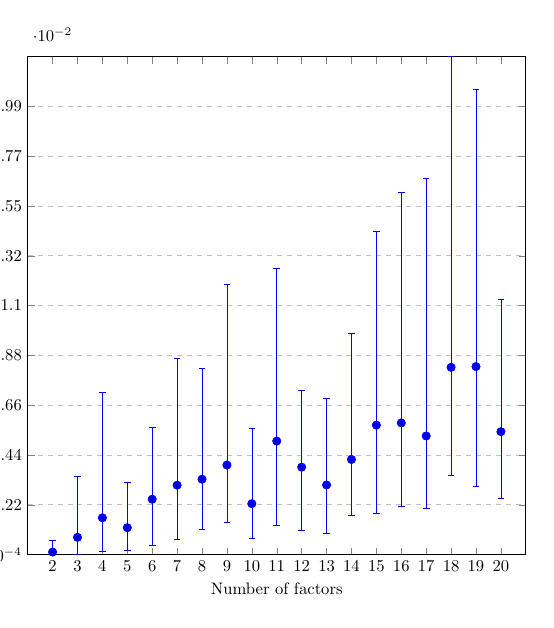
\begin{tikzpicture}[scale=0.6, trim axis left, trim axis right]
\begin{axis}[
    width=1\textwidth,
    height=1\textwidth,
    xlabel={Number of factors},
    ylabel={Time taken (s)},
    xmin=1.0, xmax=21.0,
    ymin=4e-06, ymax=0.022079,
    xticklabels={2, 3, 4, 5, 6, 7, 8, 9, 10, 11, 12, 13, 14, 15, 16, 17, 18, 19, 20},
    xtick={2, 3, 4, 5, 6, 7, 8, 9, 10, 11, 12, 13, 14, 15, 16, 17, 18, 19, 20},
    ytick={4e-06, 0.0022115, 0.004419, 0.0066265, 0.008834, 0.0110415, 0.013249, 0.0154565, 0.017664, 0.0198715},
    ymajorgrids=true,
    grid style=dashed,
]

\addplot+[
    blue,
    very thick,
    forget plot,
    only marks
    ]
    plot[
    very thick,
    error bars/.cd,
    y dir=plus,
    y explicit
    ]
    table[x=x,y=y,y error expr=\thisrow{y-max}] {
    x    y    y-max
    11	0.0050348625	0.0076751375
10	0.0022605625	0.0033444375
13	0.0030904875	0.0038565125
12	0.00387965	0.00338435
15	0.0057422625	0.0086097375
14	0.004221375	0.005607625
17	0.00526105	0.01139895
16	0.005837375	0.010202625
19	0.0083349	0.0122971
18	0.00830305	0.01377595
20	0.0054513125	0.0058676875
3	0.000769125	0.002685875
2	0.000117275	0.000506725
5	0.00119695	0.00202105
4	0.0016340375	0.0055409625
7	0.0030799625	0.0056330375
6	0.002458725	0.003203275
9	0.0039727375	0.0079962625
8	0.003345775	0.004911225

    };

\addplot+[
    blue,
    very thick,
    forget plot,
    only marks
    ]
    plot[
    very thick,
    error bars/.cd,
    y dir=plus,
    y explicit
    ]
    table[x=x,y=y,y error expr=\thisrow{y-min}] {
    x    y    y-min
    11	0.0050348625	-0.0037238625
10	0.0022605625	-0.0015505625
13	0.0030904875	-0.0021564875
12	0.00387965	-0.00278665
15	0.0057422625	-0.0039052625
14	0.004221375	-0.002456375
17	0.00526105	-0.00319205
16	0.005837375	-0.003690375
19	0.0083349	-0.0053079
18	0.00830305	-0.00477605
20	0.0054513125	-0.0029693125
3	0.000769125	-0.000737125
2	0.000117275	-0.000113275
5	0.00119695	-0.00101795
4	0.0016340375	-0.0015070375
7	0.0030799625	-0.0023959625
6	0.002458725	-0.002035725
9	0.0039727375	-0.0025607375
8	0.003345775	-0.002208775

    };

\end{axis}
\end{tikzpicture}
\vspace{-0.3cm}
\caption{Small primes, stop after one iteration}\label{fig:LenstrasEllipticCurveFactorizationsmallprimes(maximumIterations:1)factors}
\end{figure}


\begin{figure}[H]
\centering
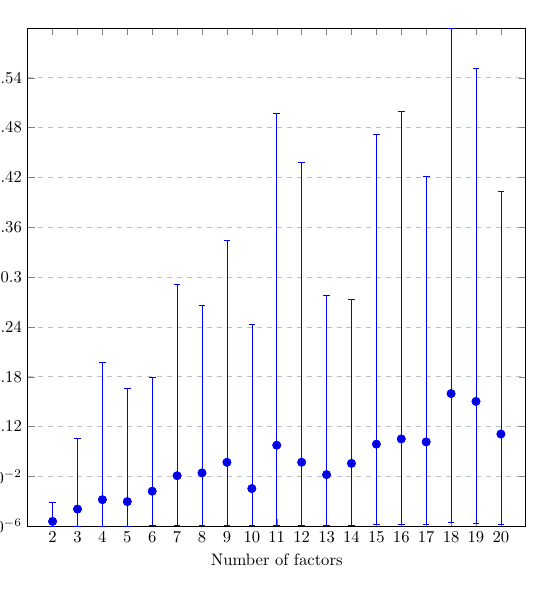
\begin{tikzpicture}[scale=0.6, trim axis left, trim axis right]
\begin{axis}[
    width=1\textwidth,
    height=1\textwidth,
    xlabel={Number of factors},
    ylabel={Time taken (s)},
    xmin=1.0, xmax=21.0,
    ymin=5e-06, ymax=0.595486,
    xticklabels={2, 3, 4, 5, 6, 7, 8, 9, 10, 11, 12, 13, 14, 15, 16, 17, 18, 19, 20},
    xtick={2, 3, 4, 5, 6, 7, 8, 9, 10, 11, 12, 13, 14, 15, 16, 17, 18, 19, 20},
    ytick={5e-06, 0.0595531, 0.1191012, 0.1786493, 0.2381974, 0.2977455, 0.3572936, 0.4168417, 0.4763898, 0.5359379},
    ymajorgrids=true,
    grid style=dashed,
]

\addplot+[
    blue,
    very thick,
    forget plot,
    only marks
    ]
    plot[
    very thick,
    error bars/.cd,
    y dir=plus,
    y explicit
    ]
    table[x=x,y=y,y error expr=\thisrow{y-max}] {
    x    y    y-max
    11	0.0967608142857	0.396752185714
10	0.0449450857143	0.196282914286
13	0.0615986857143	0.213835314286
12	0.0763987714286	0.359080228571
15	0.0980200714286	0.369938928571
14	0.0750353857143	0.195630614286
17	0.100714185714	0.317187814286
16	0.104295685714	0.391284314286
19	0.149099742857	0.398313257143
18	0.158458228571	0.437027771429
20	0.110122128571	0.289737871429
3	0.0204170571429	0.0847339428571
2	0.0057047	0.0233123
5	0.0293164285714	0.135835571429
4	0.0316512428571	0.164191757143
7	0.0603021142857	0.228674885714
6	0.0417979285714	0.135592071429
9	0.0763341	0.2652479
8	0.0636617714286	0.200044228571

    };

\addplot+[
    blue,
    very thick,
    forget plot,
    only marks
    ]
    plot[
    very thick,
    error bars/.cd,
    y dir=plus,
    y explicit
    ]
    table[x=x,y=y,y error expr=\thisrow{y-min}] {
    x    y    y-min
    11	0.0967608142857	-0.0953298142857
10	0.0449450857143	-0.0439620857143
13	0.0615986857143	-0.0603316857143
12	0.0763987714286	-0.0748697714286
15	0.0980200714286	-0.0961960714286
14	0.0750353857143	-0.0737933857143
17	0.100714185714	-0.0980221857143
16	0.104295685714	-0.102337685714
19	0.149099742857	-0.145256742857
18	0.158458228571	-0.154135228571
20	0.110122128571	-0.108252128571
3	0.0204170571429	-0.0203510571429
2	0.0057047	-0.0056997
5	0.0293164285714	-0.0289544285714
4	0.0316512428571	-0.0315432428571
7	0.0603021142857	-0.0598741142857
6	0.0417979285714	-0.0413539285714
9	0.0763341	-0.0756751
8	0.0636617714286	-0.0625907714286

    };

\end{axis}
\end{tikzpicture}
\vspace{-0.3cm}
\caption{Small Primes, Iterations:$\sqrt{n}$ }\label{fig:LenstrasEllipticCurveFactorizationsmallprimes(maximumIterations:-1)factors}
\end{figure}


The result of Lenstra's Elliptic Curve Factorization algorithm factorizing a set of large primes as seen in \ref{numbersuites}. The first plot, \ref{fig:LenstrasEllipticCurveFactorizationlargeprimes(maximumIterations:1)factors} shows the outcome of stopping Lenstra's algorithm after one iteration. The second plot, \ref{fig:LenstrasEllipticCurveFactorizationlargeprimes(maximumIterations:-1)factors} shows Lenstra's algorithm after beings topped at $\sqrt{n}$ iterations.


\begin{figure}[H]
\centering
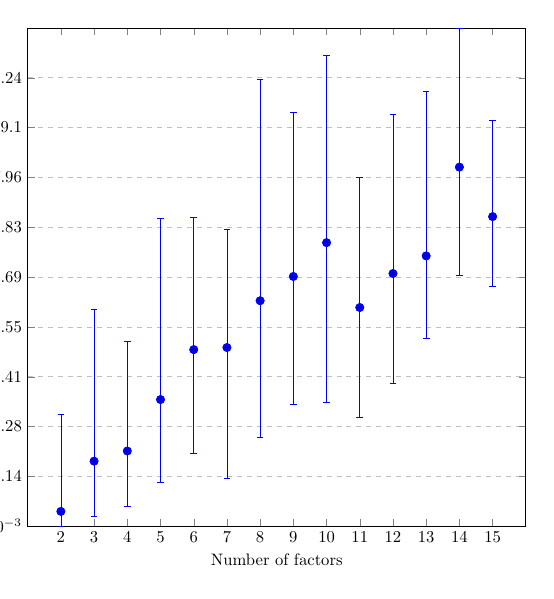
\begin{tikzpicture}[scale=0.6, trim axis left, trim axis right]
\begin{axis}[
    width=1\textwidth,
    height=1\textwidth,
    xlabel={Number of factors},
    ylabel={Time taken (s)},
    xmin=1.0, xmax=16.0,
    ymin=0.002547, ymax=11.373914,
    xticklabels={2, 3, 4, 5, 6, 7, 8, 9, 10, 11, 12, 13, 14, 15},
    xtick={2, 3, 4, 5, 6, 7, 8, 9, 10, 11, 12, 13, 14, 15},
    ytick={0.002547, 1.1396837, 2.2768204, 3.4139571, 4.5510938, 5.6882305, 6.8253672, 7.9625039, 9.0996406, 10.2367773},
    ymajorgrids=true,
    grid style=dashed,
]

\addplot+[
    blue,
    very thick,
    forget plot,
    only marks
    ]
    plot[
    very thick,
    error bars/.cd,
    y dir=plus,
    y explicit
    ]
    table[x=x,y=y,y error expr=\thisrow{y-max}] {
    x    y    y-max
    11	4.9933398	2.9658762
10	6.4743149	4.2694301
13	6.1712276	3.7602714
12	5.7694033	3.6381847
15	7.06889985714	2.20147214286
14	8.1986748	3.1752392
3	1.48588533333	3.45965266667
2	0.33928335	2.20725765
5	2.89246	4.145351
4	1.7181885	2.4993145
7	4.0801527	2.7018063
6	4.032296	3.030762
9	5.7020292	3.7549328
8	5.1483753	5.0619417

    };

\addplot+[
    blue,
    very thick,
    forget plot,
    only marks
    ]
    plot[
    very thick,
    error bars/.cd,
    y dir=plus,
    y explicit
    ]
    table[x=x,y=y,y error expr=\thisrow{y-min}] {
    x    y    y-min
    11	4.9933398	-2.5045318
10	6.4743149	-3.6536669
13	6.1712276	-1.8817726
12	5.7694033	-2.5004493
15	7.06889985714	-1.58310785714
14	8.1986748	-2.4808978
3	1.48588533333	-1.25647633333
2	0.33928335	-0.33673635
5	2.89246	-1.883798
4	1.7181885	-1.2688655
7	4.0801527	-2.9779397
6	4.032296	-2.366884
9	5.7020292	-2.9075462
8	5.1483753	-3.1277133

    };

\end{axis}
\end{tikzpicture}
\vspace{-0.3cm}
\caption{Large primes, stop after one iteration}\label{fig:LenstrasEllipticCurveFactorizationlargeprimes(maximumIterations:1)factors}
\end{figure}

\begin{figure}[H]
\centering
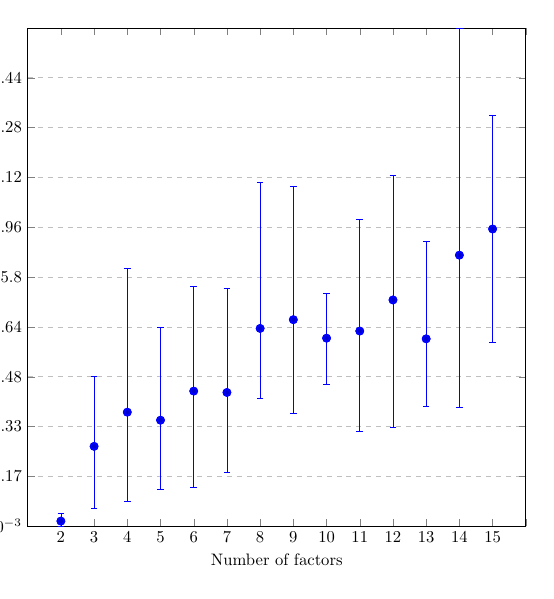
\begin{tikzpicture}[scale=0.6, trim axis left, trim axis right]
\begin{axis}[
    width=1\textwidth,
    height=1\textwidth,
    xlabel={Number of factors},
    ylabel={Time taken (s)},
    xmin=1.0, xmax=16.0,
    ymin=0.006143, ymax=11.600464,
    xticklabels={2, 3, 4, 5, 6, 7, 8, 9, 10, 11, 12, 13, 14, 15,},
    xtick={2, 3, 4, 5, 6, 7, 8, 9, 10, 11, 12, 13, 14, 15, 16, 17, 18, 19, 20},
    ytick={0.006143, 1.1655751, 2.3250072, 3.4844393, 4.6438714, 5.8033035, 6.9627356, 8.1221677, 9.2815998, 10.4410319},
    ymajorgrids=true,
    grid style=dashed,
]

\addplot+[
    blue,
    very thick,
    forget plot,
    only marks
    ]
    plot[
    very thick,
    error bars/.cd,
    y dir=plus,
    y explicit
    ]
    table[x=x,y=y,y error expr=\thisrow{y-max}] {
    x    y    y-max
    11	4.5472213	2.5943217
10	4.3813821	1.0425829
13	4.3661165	2.2646215
12	5.2711618	2.8968452
15	6.9222887	2.6438803
14	6.3138906	5.2865734
3	1.863128	1.640782
2	0.1234448	0.1778742
5	2.4723056	2.1704004
4	2.6590272	3.3385778
7	3.117723	2.416449
6	3.1491498	2.4300842
9	4.8116204	3.1010296
8	4.608257	3.398077

    };

\addplot+[
    blue,
    very thick,
    forget plot,
    only marks
    ]
    plot[
    very thick,
    error bars/.cd,
    y dir=plus,
    y explicit
    ]
    table[x=x,y=y,y error expr=\thisrow{y-min}] {
    x    y    y-min
    11	4.5472213	-2.3403543
10	4.3813821	-1.0745521
13	4.3661165	-1.5725185
12	5.2711618	-2.9638238
15	6.9222887	-2.6459547
14	6.3138906	-3.5397636
3	1.863128	-1.432919
2	0.1234448	-0.1173018
5	2.4723056	-1.6200266
4	2.6590272	-2.0718492
7	3.117723	-1.859811
6	3.1491498	-2.2341108
9	4.8116204	-2.1788084
8	4.608257	-1.617636

    };

\end{axis}
\end{tikzpicture}
\vspace{-0.3cm}
\caption{Large primes, stop after $\sqrt{n}$ iterations}\label{fig:LenstrasEllipticCurveFactorizationlargeprimes(maximumIterations:-1)factors}
\end{figure}

